
\section{Numerical Integration} \label{background}
The basic problem in numerical integration is to compute an approximate solution to a definite integral of the form of formula \ref{integral}, to a given degree of accuracy which depends on the application \cite{Wiki_Integration}. This section presents the main approaches to numerical integration. The choice depends mainly on the present data or function and on the results required \cite{Dalziel1998, Espelid}.



\subsection{Manual Method - Counting Squares}
One of the simpler but inexact methods for determining the area below a figure is \emph{integration by hand}. The basic idea of this approach is to superimpose a grid with a known size on the graph of the function to be integrated and count the squares which are covered by more than $50\%$ of the function. This approach is visualized in figure \ref{fig:manual_integration}. The finer the grid is chosen, the more accurate is the result. Another way to improve accuracy is to use triangles or other shapes instead of squares in the border area. \cite{Dalziel1998}

\begin{figure}[htbp]
	\centering
		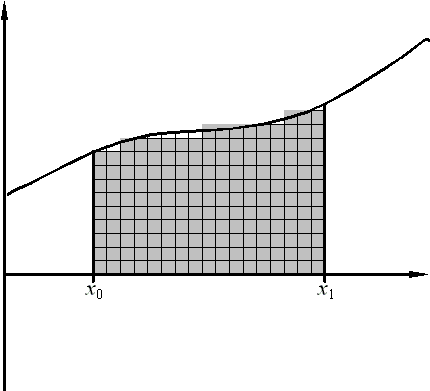
\includegraphics[width=0.4\textwidth]{graphics/manual}
	\caption{Manual method for determining the area below a graph. The grey squares are the ones which are by more than 50\% inside and thus are counted.}
	\label{fig:manual_integration}
\end{figure}


\subsection{Midpoint Rule}
The idea of the midpoint rule, which is also called \emph{rectangle method}, is to approximates the integral over an interval $[a, b]$ by calculating the area of a corresponding rectangle (see figure \ref{fig:midpoint_rule}). This rectangle has width $b-a$ and height $f(c)$ with $c=\frac{a+b}{2}$ being the midpoint. Thus the integral can be approximated with equation \ref{eq:midpoint_rule}. This rule is exact for polynomials with one degree, namely constant and linear functions. \cite{Wiki_Rectangle}

\begin{equation}
\int\limits_{a}^{b} f(x)\, dx \approx (b - a) \cdot f(c) = (b - a) \cdot f\!\left(\frac{a + b}{2}\right)
 \label{eq:midpoint_rule}
\end{equation}



\begin{figure}[hb]
\centering
\begin{minipage}{.45\textwidth}
  \centering
	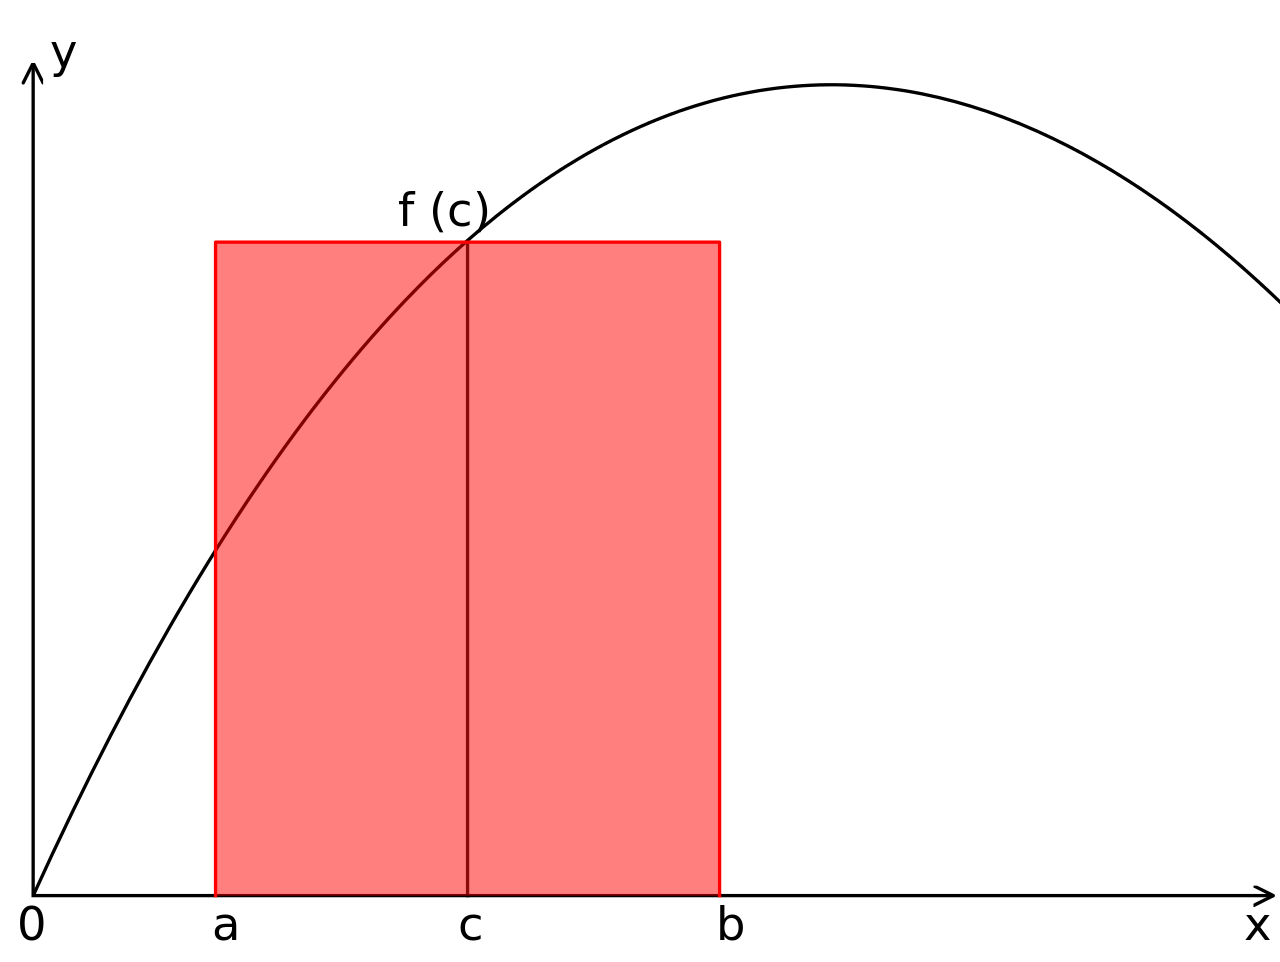
\includegraphics[width=0.9\textwidth]{graphics/midpoint.png}
	\caption{Midpoint Rule. Approximation of the integral by constructing a rectangle with height $f(c)$.}
	\label{fig:midpoint_rule}  
\end{minipage} \hspace{10px}
\begin{minipage}{.45\textwidth}
  \centering
  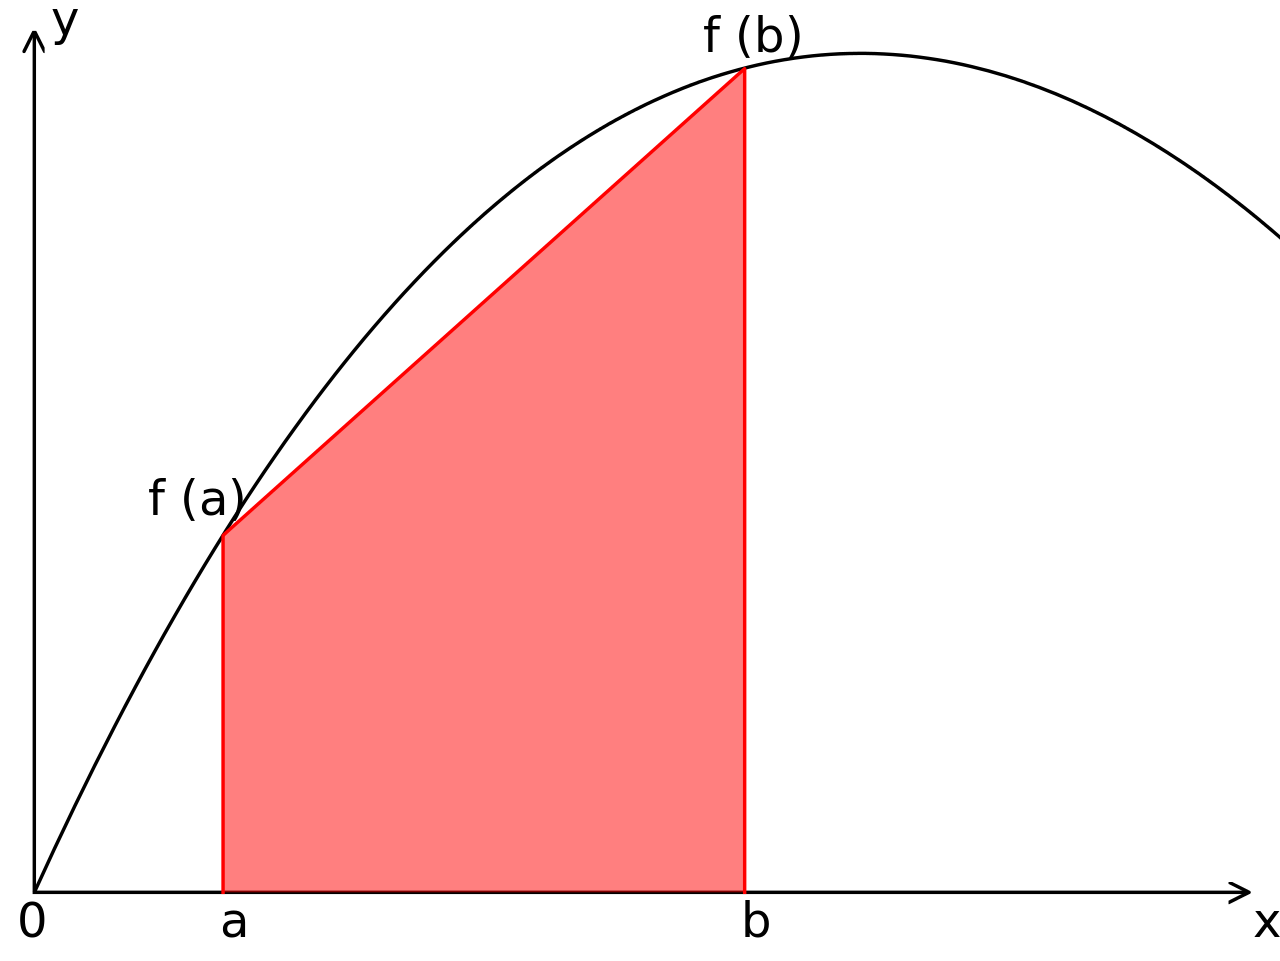
\includegraphics[width=0.9\textwidth]{graphics/trapezoid3}
	\caption{Trapezoid Rule.\newline Approximation of the integral by constructing a trapezoid from $f(a)$ to $f(b)$. }
	\label{fig:trapez_integration}
\end{minipage}
\end{figure}

\subsection{Trapezoid Rule}
The trapezoid rule uses a similar concept as the Midpoint rule. It approximates the integral of a function by the area of a trapezoid as shown in figure \ref{fig:trapez_integration}. The trapezoid itself has base $h = b - a$ and sides equal to the values of the integrand at the two endpoints $a$ and $b$. Thus, the integral of a function can be approximated by equation \ref{eq:trapezoid_rule}. Again, this rule is exact for constant and linear functions but provides better approximations for functions of a higher degree, compared to the midpoint rule.

\begin{equation}
 \int_{a}^{b} f(x)\, dx \approx (b-a) \left[\frac{f(a) + f(b)}{2} \right]
 \label{eq:trapezoid_rule}
\end{equation}



\subsection{Composite Rules}
Although the previous rules are exact for constant and linear functions, one cannot expect neither the midpoint nor the trapezoid rule to give accurate results for polynomials of a higher degree over a large interval. Therefore the idea is to split the main interval into $n$ short sub-intervals and compute an approximation for each sub-interval as shown in figure \ref{fig:trapez_composite}. Summing up those partial results gives a better approximation of the integral over the whole interval. This is called the composite rule. \cite{Skokos2010}

\begin{figure}
\centering
  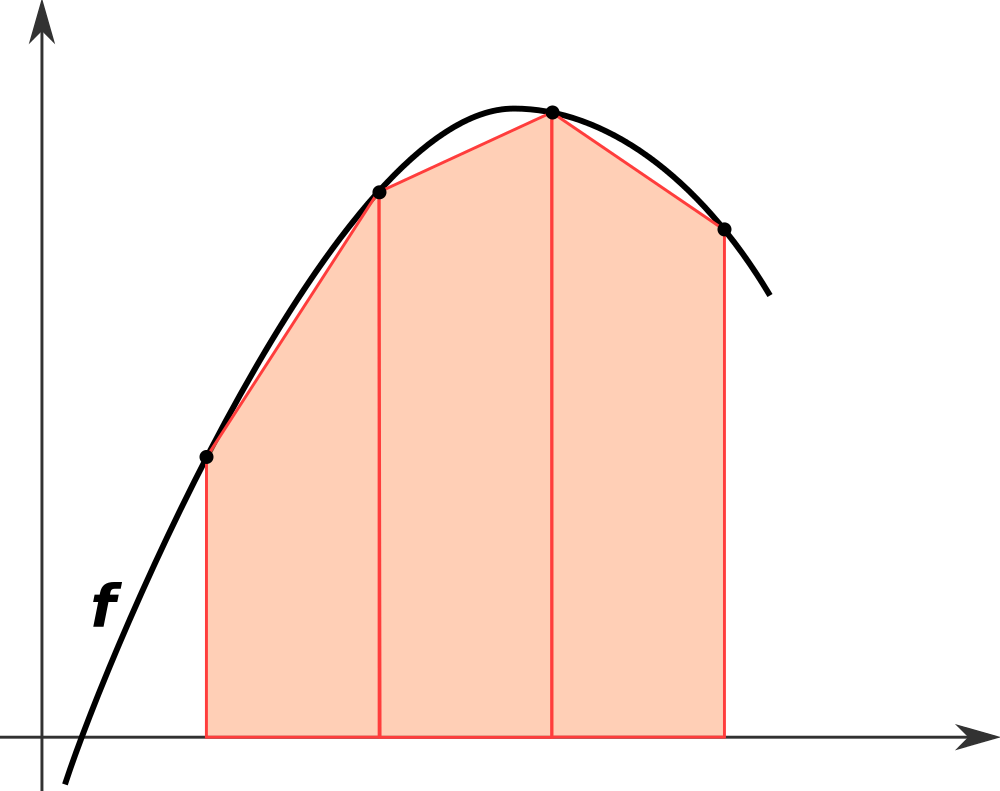
\includegraphics[width=0.5\textwidth]{graphics/trapez_composite.png}
	\caption{Trapezoid composite rule}
	\label{fig:trapez_composite}
\end{figure}


As $n$ gets larger, the intervals become smaller and the computation of the integral gets more accurate. This idea is the spirit of the definition of the Riemann integral and the limit of this approximation as n $\to \infty$ is defined and equal to the integral $\int_{a}^{b}\, f$, if this Riemann integral is defined. \cite{Wiki_Rectangle}

Comparing the midpoint and trapezoid rule, there are two advantages of the former one. First, there are less function evaluations needed to approximate the integral which can matter. Second it can be used more effectively for determining the integral near an integratable singularity since endpoints are not used, only a point inside the interval. \cite{Dalziel1998}

However, an analysis of Weidemann \cite{Weideman2002} shows that the trapezoid rule becomes extremely accurate when integrating periodic functions. He concludes that 'Using more sophisticated rules may not be worth the effort'.



\subsection{Simpsons's Rule}

The idea of the Simpson's rule is to use a parabola to approximate the integrand. This increases the accuracy of the approximation without a need to decrease the step size as much as it would be necessary with some lower order polynomial. The Simpson's rule provides exact results for any polynomial of degree three or less. The name of this rule comes from the English mathematician Thomas Simpson but since Kepler used similar formulas more than a century before, it sometimes is also called the Kepler's rule or Keplersche Fassregel. \cite{Wiki_Simpsons}

\begin{equation}
 \int_{a}^{b} f(x) \, dx \approx \tfrac{b-a}{6}\left[f(a) + 4f\left(\tfrac{a+b}{2}\right)+f(b)\right]
\label{eq:simpsons}
\end{equation}

Although this rule provides better results, approximating a function which is highly oscillatory or which lacks derivatives at certain points, the results may be still very poor. To increase the accuracy this function can also be used on sub-intervals and is then called the \emph{Composite Simpson's Rule}.

Formula \ref{eq:simpsons} is derived by evaluating the function at the two boundary points $a$ and $b$ of the interval, plus the midpoint $m = \frac{a+b}{2}$, see figure \ref{fig:Simpsons_rule2}. 

\begin{figure}[htbp]
	\centering
		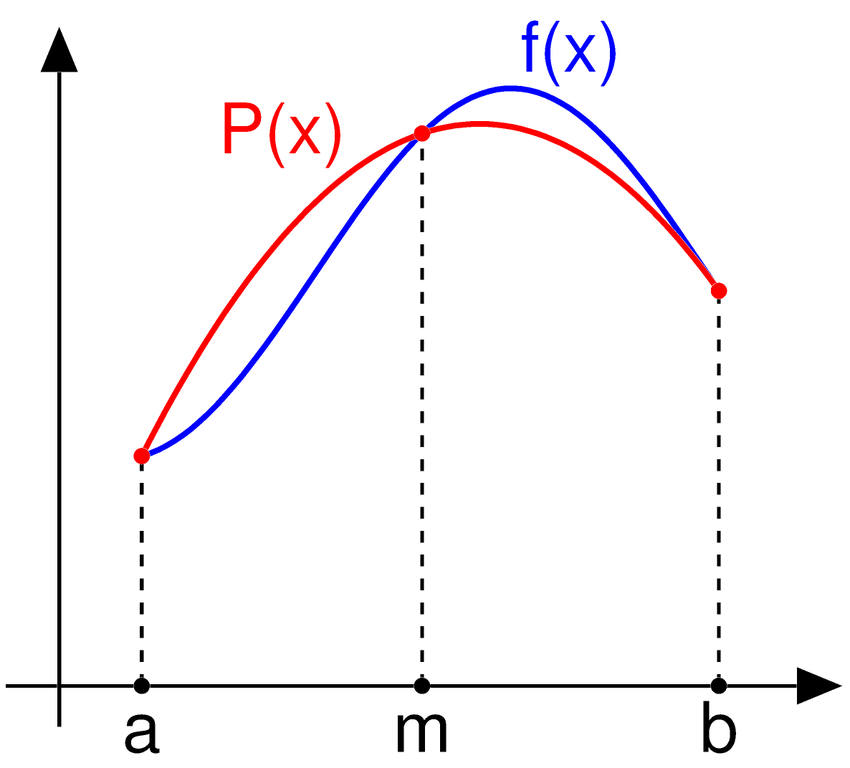
\includegraphics[width=0.40\textwidth]{graphics/simpsons2.png}
	\caption{Simpsons Rule. Using three points to interpolate a polynomial $p(x)$ in order to approximate $f(x)$.}
	\label{fig:Simpsons_rule2}
\end{figure}



\subsection{Newton-Cotes formulas}
When looking at the rules which are presented so far, it can be observed, that all rules have a general form, which is shown in equation \ref{eq:nq}. The points $x_i$ are always equally spaced and the rules only differ in the number of function points which are used for the approximation. Their corresponding weights $w_i$ are derived from Lagrange basis polynomials. An advantage of equal spacing is, that values can be reused which can minimizes the computational overhead.
\begin{equation}
\int_a^b f(x) \,dx \approx w_0 f(x_0) + w_1 f(x_1) + \dots + w_n f(x_n) = \sum_{i=0}^n w_i\, f(x_i)
\label{eq:nq}
\end{equation}

Equations \ref{eq:nq_mid}, \ref{eq:nq_trap} and \ref{eq:nq_simp} exemplary show the corresponding points $x_i$ and their weights.

\begin{equation}
\text{Midpoint:} \quad  x = \frac{a + b}{2}, \quad w = 1
\label{eq:nq_mid}
\end{equation}

\begin{equation}
\text{Trapezoid:} \quad x_0 = a, x_1 = b, \quad w_0 = w_1 = \frac{b-a}{2}
\label{eq:nq_trap}
\end{equation}

\begin{equation}
\text{Simpson's:}
\quad x_0 = a, x_1 = \frac{a+b}{2}, x_2 = b, 
\quad w_0 = w_2 = \frac{b-a}{6}, w_1 = 4 * \frac{b-a}{6}
\label{eq:nq_simp}
\end{equation}

There are two types of Newton-Cotes formulas, open and closed ones. While the former only uses the points in between the interval (for example the midpoint rule), the closed formulas (such as the Simpson's rule) also use the function values at the endpoints. Newton-Cotes formulas of any higher degree $n$ can be constructed as well. \cite{Wiki_Cotes} 


\subsection{Gaussian Quadrature}\label{sec:gauss_quad}
The main idea of the Gaussian quadrature is to not use equally spaced intervals at which the function is evaluated but to carefully choose the points $x_i$ and their weights to maximize accuracy. Thereby, the general form of the rule stays the same as for the Newton-Cotes rule (equation \ref{eq:nq}) but the $x_i$ and weights differ. There exist multiple forms of the Gaussian quadrature while the Gauss-Legende quadrature is the most known one. In general, the result of a rule which uses $n$ points is exact for polynomials of degree $2n-1$ or less. The Gauss-Legendre quadrature is by default defined over the interval $[-1, 1]$ so that an integral over an interval $[a, b]$ must be changed before the Gaussian quadrature rule can be applied. A change of interval can be done as shown in equation \ref{eq:interval}. However, there are other forms which are defined over other intervals. Although the computational overhead is slightly higher compared to the Newton-Cotes rules, the Gaussian quadrature rules are typically more accurate.  \cite{wiki:gauss}

Table \ref{tab:gauss_quad} shows some low order Gaussian-Legendre rules up to a degree of $5$.


\begin{equation}
\int_a^b f(x)\,dx = \frac{b-a}{2} \int_{-1}^1 f\left(\frac{b-a}{2}x + \frac{a+b}{2}\right)\,dx
\label{eq:interval}
\end{equation}


\newcommand{\specialcell}[2][c]{%
  \begin{tabular}[#1]{@{}c@{}}#2\end{tabular}}
\begin{table}[htbp]
\centering
\caption{Parameters for low order Gaussian-Legendre quadrature}
\begin{tabular}{|c|c|c|}
\hline
Number of points, $N$ & Points, $X_i$   & Weights, $w_i$   \\ \hline

1                   & 0               & 2               \\ \hline

2                   & 
$\pm \sqrt{\frac{1}{3}}$ & 1               \\ \hline

3                   
& \specialcell{$0$ \\ $\pm \sqrt{\frac{3}{5}}$}       
& \specialcell{$\frac{8}{9}$ \\ $\frac{5}{9}$} \\ \hline

4                   
& \specialcell{$\pm\sqrt{\tfrac{3}{7} - \tfrac{2}{7}\sqrt{\tfrac{6}{5}}}$
		\\ $\pm\sqrt{\tfrac{3}{7} + \tfrac{2}{7}\sqrt{\tfrac{6}{5}}}$}
& \specialcell{$\tfrac{18+\sqrt{30}}{36}$ \\ $\tfrac{18-\sqrt{30}}{36}$}  \\ \hline

5                   
& \specialcell{$0$ \\ $\pm\tfrac13\sqrt{5-2\sqrt{\tfrac{10}{7}}}$
		\\ $\pm\tfrac13\sqrt{5+2\sqrt{\tfrac{10}{7}}}$}
& \specialcell{$\tfrac{128}{225}$ \\ 
			$\tfrac{322+13\sqrt{70}}{900}$ \\ 
			$\tfrac{322-13\sqrt{70}}{900}$}  \\ \hline


\end{tabular}
\label{tab:gauss_quad}
\end{table}



% \subsection{Romberg Integration}

\subsection{Monte Carlo Method}
A method which does not use an approximation formula is the Monte Carlo method. Instead the integral is determined by randomly choosing $n$ points over the integration interval $[a, b]$. The integral is then approximated by the average over the function values at those random points (equation \ref{eq:montecarlo}).

\begin{equation}
\int_a^b f(x) \,dx \approx\frac {b-a}n \sum_{i=1}^n f(x_i)
\label{eq:montecarlo}
\end{equation}

The advantage of this approach is its easy implementation and extensibility, especially on multidimensional integrals. However, the computation time is higher compared to other approximation formulas. Moreover, Monte Carlo does not always provide $100\%$ correctness but in general the results will be correct. \cite{Robert2010, Judd2011}



\subsection{Multidimensional Integrals} 

When trying to estimate the value of multidimensional integrals, a distinction between cases of low and high dimensionality has to be made \cite{NAGlib}. Where the number of dimensionalities is lower than 4 or 5, one- dimensional methods, such as the ones mentioned above, may be applied to each dimension, according to some suitable strategy. However, special techniques are needed for integrals of higher dimensionality since the  number of evaluation rises very rapidly with the number of dimensions. Therefore non deterministic approaches such as the \emph{Monte-Carlo} method, which randomly chose the points at which the integrand is evaluated, can be used.